\documentclass[UTF8]{ctexart}
\usepackage{mathtools,booktabs}
\usepackage{graphicx}
%添加路径,图片的搜索路径
\graphicspath{{figures/}}
\usepackage{listings} 
\usepackage{xcolor}
\lstset{
	language=c,  %代码语言使用的是matlab
	frame=shadowbox, %把代码用带有阴影的框圈起来
	rulesepcolor=\color{red!20!green!20!blue!20},%代码块边框为淡青色
	keywordstyle=\color{blue!90}\bfseries, %代码关键字的颜色为蓝色,粗体
	commentstyle=\color{red!10!green!70}\textit,    % 设置代码注释的颜色
	showstringspaces=false,%不显示代码字符串中间的空格标记
	numbers=left, % 显示行号
	numberstyle=\tiny,    % 行号字体
	stringstyle=\ttfamily, % 代码字符串的特殊格式
	breaklines=true, %对过长的代码自动换行
	extendedchars=false,  %解决代码跨页时,章节标题,页眉等汉字不显示的问题
	%   escapebegin=\begin{CJK*},escapeend=\end{CJK*},      % 代码中出现中文必须加上,否则报错
	texcl=true}


\begin{document}
	
	\title{八股文背诵合集}
	\author{The Sea}
	\maketitle
	
	\tableofcontents
	\newpage
	
	\section{Spring}
	%\subsection{二级标题}
	\subsubsection{Spring 框架能带来哪些好处}

	\begin{enumerate}
		\item Dependency Injection(DI) 依赖注入 是的构造器和JavaBean properties文件中的依赖关系一目了然.
		\item IoC容器更加趋向于轻量级.
	\end{enumerate}
	
	\subsubsection{什么是控制反转(IOC)}
	\begin{enumerate}
		\item 
		控制反转简单来说, 以前程序开发的时候, 是由程序员通过new来生成对象. 在使用控制反转的情况下, 对象的实例化由Spring框架中的IoC容器来控制对象的创建; 
		\item 由容器来管理这些对象的生命周期.
		\item Spring中的org.springframework.beans包和org.springframework.conext包构成了Spring框架Ioc的基础. 主要使用文件 applicationContext.xml 来进行配置.
	\end{enumerate}

	\subsubsection{什么是依赖注入?}
	\begin{enumerate}
		\item Spring 通过反射来实现依赖注入
		\item 当我们需要某个功能比如Connection, 至于Connection怎么构造, 何时构造我们不需要知道. 在系统运行时, Spring会在适当的时候制造一个Connection, 我们需要一个Connection, 这个Connection是由Sping注入到A中. 
	\end{enumerate}
	
	\subsubsection{第三个三级标题}
	
	
	\section{java基础}
	%\subsection{二级标题}
	\subsubsection{快速失败(fail-fast) 和 安全失败(fail-safe) 的区别是什么?}
	\begin{enumerate}
		\item java.util包下面的所有的集合类都是快速失败的, 而java.util.concurrent包下面的所有类都是安全失败的. 快速失败的迭代器会抛出ConcurrentModificationException异常, 而安全失败的迭代去永远不会抛出这样的异常.

	\end{enumerate}

	\subsubsection{hashmap的数据结构}
	\begin{enumerate}
		\item jdk1.7 由 数组 + 链表  来构成
		\item jdk1.8 由 数组 + 链表 + 红黑树 来构成
		\item jdk1.8的时候, 当元素不超过64个的时候, 不会出现链表转红黑树, 当元素超过64个的时候, 会出现链表转红黑树.
		\item jdk1.8 当链表长度达到8个的时候, 链表会转为红黑树, 当红黑树元素长度退回到6个的时候会出现红黑树转为链表.
		\item jdk1.7 采用头插法, jdk1.8采用尾插法.
	\end{enumerate}
	\subsubsection{heap和stack有什么区别}
	\begin{enumerate}
		\item java的内存分为两类, 一类是堆内存, 一类是栈内存
		\item 栈内存是指程序进入一个方法时, 会为这个方法单独分配一块私属存储空间, 用于存储这个方法内部的局部变量. 当这个方法结束时, 分配给这个方法的栈会释放, 这个栈中的变量也随之释放.
		\item 使用new创建的对象存放在堆里, 不会随方法的结束二小时. 方法中的局部变量使用final修饰后, 放在堆中, 而不是栈中.
		
	\end{enumerate}

	\subsubsection{Array 和 ArrayList 的区别}
	\begin{enumerate}
		\item Array 大小固定, ArrayList 大小是动态变化的.
	\end{enumerate}
	\subsubsection{Collection 和 Collections 的区别}
	\begin{enumerate}
		\item Collection 是集合类的上级接口, 继承他的接口主要是set和list
		\item Collections 类数针对集合类的一个帮助类. 它提供了一系列的静态方法对各种集合的搜索, 排序, 线程安全化等操作.
	\end{enumerate}


\section{JVM}
%\subsection{二级标题}
\subsubsection{GC的三种收集方法: 标记清除, 标记整理, 复制算法的原理与特点, 分别用在什么地方, 如果让你优化收集方法, 有什么思路}
\begin{enumerate}
	\item 标记清除: 先标记, 标记完毕之后再清除, 缺点: 效率不高会产生碎片.
	\begin{figure}
		\centering
		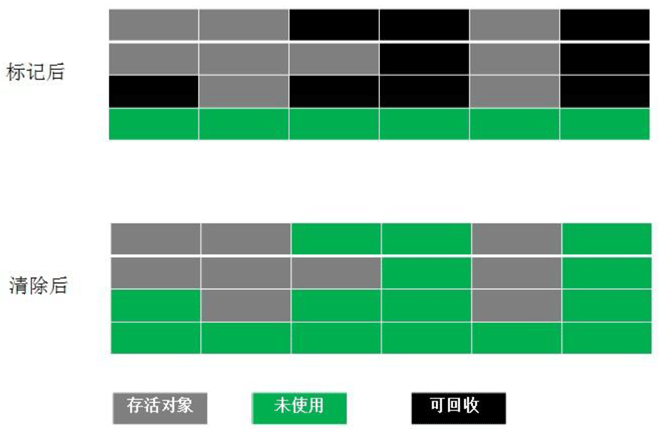
\includegraphics[width=0.7\linewidth]{figures/sign_remove.png}
		\caption{}
		\label{fig:sign_remove}
	\end{figure}
	\item 标记整理: 标记完毕之后, 让所有存活的对象向一端移动
	\item 复制算法: 分别8:1的Eden去和survivor区
	\begin{figure}
		\centering
		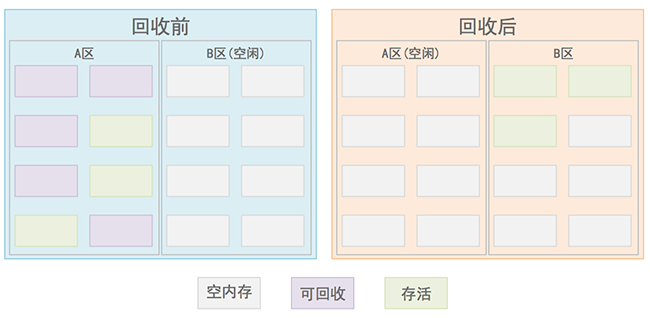
\includegraphics[width=0.7\linewidth]{figures/jvm_copy.jpg}
		\caption{}
		\label{fig:jvm_copy}
	\end{figure}
\end{enumerate}
\subsubsection{JVM的主要组成部分及其作用?}
JVM包含两个子系统和两个组件, 两个子系统为Class loader(类加载), Execution engin(执行引擎); 两个组件为 Runtime data area(运行时数据区), native Interface(本地接口)

\begin{enumerate}
	\item Class loader: 根据给定的额全限定类名(如:java.lang.object)来装在class文件到Runtime data area中的method area.
	\item Execution engine(执行引擎): 执行classes中的指令
	\item native Interface(本地接口): 与native libraries交互, 是其他编程语言交互的接口.
	\item Runtime data area(运行时数据区): 这就是我们常说的jvm的内存
\end{enumerate}
\par
\textbf{作用:} 首先通过编译器吧java代码转换成字节码, 类加载器(ClassLoader) 再把字节码加载到内存中, 将其放在运行时数据区(Runtime data area)的方发区内, 而字节码文件知识jvm的一套指令集规范, 并不能直接交给底层操作系统去执行, 因此需要特定的命令解析器执行引擎(Execution Engine), 将字节码翻译成底层系统指令, 在交由CPU去执行, 而这个过程中需要调用其他语言的本地库接口(Native Interface) 来实现整个程序的功能. 
\par
Java程序运行机制步骤
\begin{enumerate}
	\item 编码: IDEA等IDE进行编码java, 后缀.java
	\item 编译: javac 将源代码编译成字节码文件,字节码文件的后缀名为.class
\end{enumerate}
类的加载是将类的.class文件中的二进制数据读入到内存中, 将其放在运行时数据区的方法去内, 然后在堆区创建一个java.lang.Class对象, 用来封装类在方区内的数据结构.
\subsubsection{JVM运行时数据区}
运行时数据区由如下几个区域构成
\begin{enumerate}
	\item 程序计数器(PC): 当前线程所执行字节码的行号指示器, 字节码解析器的工作是通过改变这个计数器的值, 来选去下一条需要执行的字节码指令.
	\item java虚拟机栈(Java Virtual Machine Stacks): 用于存储局部变量表, 操作数栈, 动态链接, 方法出口等信息.
	\item 本地方法栈(Native Method Stack) : 与虚拟机栈的作用是一样的, 只不过虚拟机栈是服务Java方法的, 而本地方法栈是为虚拟机调用Native方法服务的.
	\item Java堆(Java Heap): Java 虚拟机中内存最大的一块, 是被所有线程共享的, 几乎所有的对象实例, 都在这里分配内存;
	\item 方法区(Method Area): 用于存储已被虚拟机加载的类信息, 常量, 静态变量, 及时编译后的代码等数据.
\end{enumerate}
\subsubsection{说一下堆栈的区别?}
\textbf{物理地址}
\par
堆的物理地址分配对对象是不连续的. 因此, 性能慢些. 在GC的时候也要考虑到不连续的分配, 所以后各种算法. 比如, 标记-清除, 复制, 标记压缩, 分代(即新生代生活复制算法, 老年代使用标记压缩算法);
\par
栈使用的是数据结构中的栈, 先进后出的原则, 物理地址分配是连续的. 所以性能快.
\par
\textbf{内存区别}
\par
堆因为是不连续的, 所以分配的内存是在\textbf{运行期}确认的, 因此大小不固定. 一般堆大小远大于栈.
\par
栈是连续的, 所以分配的内存大小要在编译器就确认, 大小是固定的.
\par
\textbf{程序的可见度}
\par
堆对于整个应用程序都是共享, 可见的.
栈只对于线程是可见的. 所以也是线程私有. 他的生命周期和线程相同.
TIPS:
\begin{enumerate}
	\item 静态变量放在方法区.
	\item 静态的对象还是放在堆.
\end{enumerate}

\subsubsection{对象的访问定位?}
目前主流的访问方式有句柄和直接指针两种方式.

\begin{enumerate}
	\item 指针: 指向对象, 代表一个对象再内存中的起始地址
	\item 句柄: 可以理解为指向指针的指针, 维护者对象的地址. 句柄不直接指向对象, 而是指向对象的地址(句柄不发生变化, 指向固定内存你地址), 再由对象的指针指向对象的真实内存地址.
\end{enumerate}
\textbf{句柄访问}
\par
Java堆中划分出一块内存作为句柄池, 引用中存储对象的句柄地址, 而句柄中包含了\textbf{对象实例数据}与\textbf{对象类型数据}各自的决堤地址信息, 具体构造如下图所示:
\begin{figure}
	\centering
	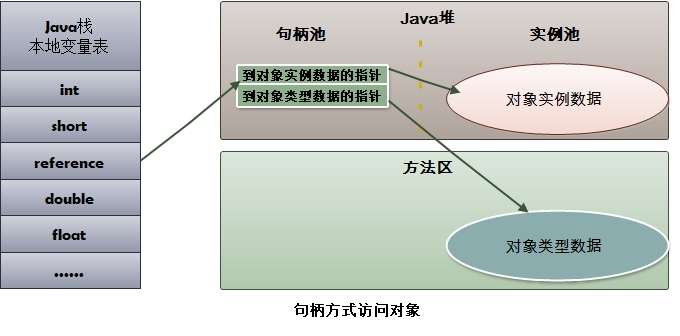
\includegraphics[width=0.7\linewidth]{figures/jvm_handler.jpg}
	\caption{}
	\label{fig:jvm_handler}
\end{figure}
\textbf{直接指针}
\par
\begin{figure}
	\centering
	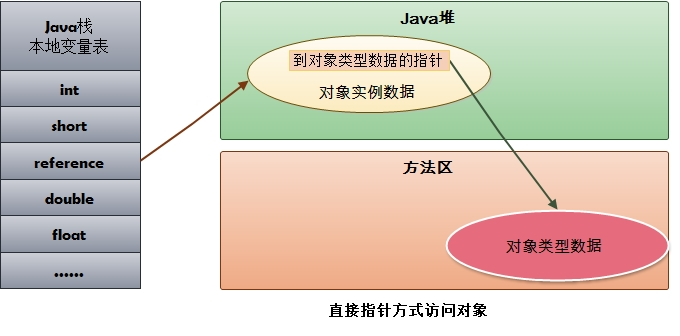
\includegraphics[width=0.7\linewidth]{figures/jvm_point.jpg}
	\caption{}
	\label{fig:jvm_point}
\end{figure}
\subsubsection{垃圾回收器的基本原理是什么?}
\textbf{可达性分析}
\par
GC采用有向图的方式记录和管理堆中的所有对象. 通过这种方式确定哪些对象是"可达的", 哪些对象是"不可达的", 当GC确定一些对象为"不可达"时, GC就有责任回收这些内存空间.
程序员可以手动执行System.gc(), 通知GC运行, 但是Java语言规范并不保证GC一定会执行.
\par
\textbf{引用计数法}
为每个对象创建一个引用技术, 有对象引用时计数器+1, 引用被释放是技术-1, 当计数器为0时就可以被回收. 优缺点, 不能解决循环引用的问题.
\subsubsection{在java中, 对象什么时候可以被垃圾回收?}
当对象边的不可触及的时候, 这个对象就可以被回收了, 垃圾回收不会发生在永久代, 如果永久代满了或者是超过了临界值, 会触发完全垃圾回收(full gc), 会导致Stop-the-world. 
	\section{Redis}
	%\subsection{二级标题}
	\subsubsection{什么是Redis?}
	\begin{enumerate}
		\item 高性能非关系型数据库
		\item 可以存储五种不同类型的额值之间的映射. 键的类型只能为字符串, 值支持五种类型数据:字符串, 列表, 集合, 散列表, 有序集合.
		\item redis数据是存在内存中的, 所以读写速度非常快.
		
	\end{enumerate}
	\subsubsection{AOF和RDB两种持久化方式区别}
	\begin{enumerate}
		\item AOF存储命令, RDB存储数据.
		\item AOF文件因为存储命令, 所以在redis启动的时候加载aof会比加载rdb要慢. 
	\end{enumerate}
	\subsubsection{为什么要使用Redis}
	\begin{enumerate}
		\item 高性能: 内存的读取比硬盘乃至固态硬盘的读取速度都要快得多
		\item 高并发: 直接操作缓存能够承受的请求是远远大于直接访问数据库的, 所以我们可以考虑把数据库中的部分数据转移到缓存中去, 这样用户的一部分请求会直接请求缓存这里而不用经过数据库. 
		\item 高性能: 使用多路I/O复用木星, 非阻塞IO;
	\end{enumerate}
	\subsubsection{为什么要使用Redis而不用map/guavaCache做缓存}
	\begin{enumerate}
		\item guavaCache实现的是本地缓存, 最主要的特点是轻量化以及快速, 生命周期随着jvm的销毁而结束, 冰洁在多实例的情况下, 每个实例都需要个字保存一份缓存, 缓存容易出现不一致性.
		\item 使用redis之类的缓存称为分布式缓存, 在多实例的情况下, 各实例公用一份缓存数据, 缓存具有一致性.
	\end{enumerate}
	\subsubsection{分布式锁如何使用redis实现}
	\begin{enumerate}
		\item setnx命令原子性实现. 
	\end{enumerate}
	\subsubsection{Redis的内存淘汰策略有哪些}
	Redis的内存淘汰策略是指在Redis用于缓存的内存不足时, 怎么处理需要新写入且需要申额外空间的数据.
	全局的键空间选择性移除
	\begin{enumerate}
		
		\item noeviction: 当内存不足以容纳新写入数据时, 新写入操作会报错.
		\item allkeys-lru: 当内存不足以容纳新写入数据时, 在键空间中, 移除最近最少使用的key.
		\item allkeys-random: 当内存不足以容纳新写入数据时, 在键空间随机移除某个key.
	\end{enumerate}
	设置过期时间的键空间选择性移除
	\begin{enumerate}
		
		\item volatile-lru: 当内存不足以容纳新写入数据时, 在设置了过期时间的键空间中, 移除最近最少使用的key.
		\item volatile-random: 当内存不足以容纳新写入数据时, 在设置了过期时间的键空间中, 随机移除某个key.
		\item volatile-ttl: 当内存不足以容纳新写入的数据时, 在设置了过期时间的键空间中, 有更早过期时间的key优先移除. 
	\end{enumerate}
	\subsubsection{Redis事物的概念}
	Redis事物的本质通过MULTI, EXEC, WATCH等一组命令的集合. 
	\begin{enumerate}
	
		\item 事物开始 MULTI
		\item 命令入队
		\item 事务执行 EXEC
	\end{enumerate}
* 事务执行过程中, 如果服务端收到有EXEC, DISCARD, WATCH, MULTI之外的请求, 将会把请求放入队列中排队.
简单介绍一下watch, 当watch的变量在事务过程中发生了改变, 那么事务失败, 拒绝执行事物.
\begin{lstlisting}
	>watch 'name'
	>multi
	>set "name" "peter"
	>exec
	(nil)
\end{lstlisting}
\subsubsection{RedisSharding}
简单来说就是多个client 连接多个redis, 然后通过一致性哈希算法, 来确定访问的key+访问的客户端名字在哪一台redis上.
采用的算法是MURMUR\_HASH, 
\begin{figure}
	\centering
	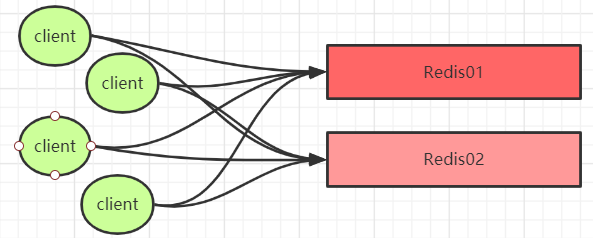
\includegraphics[width=0.7\linewidth]{figures/redis_sharding.png}
	\caption{}
	\label{fig:redissharding}
\end{figure}
\subsubsection{缓存雪崩}
缓存同一时间大面积的失效, 所以, 后面的请求都会落到数据库上, 造成数据库短时间内承受大量请求而崩掉

\par
\textbf{解决方案}
\begin{enumerate}
	
	\item 缓存数据的过期时间设置随机, 防止同一时间大量数据过期现象发生.

\end{enumerate}

\subsubsection{缓存穿透}
缓存和数据库中都没有数据, 导致所有的请求都落在数据库中, 造成数据库短时间内承受大量请求而崩掉.
\par
\textbf{解决方案}
\begin{enumerate}
	
	\item 从缓存中取不到的数据, 在数据库中也没有取到, 这时也可以将key-value对写为key-null, 缓存时间设定为30s.
	
\end{enumerate}

\subsubsection{缓存击穿}
缓存中没有但数据库中有的数据, 由于并发用户特别多, 同时读缓存没读到数据, 又同时去数据库取数据, 引起数据库压力瞬间增大, 造成过大压力, 和缓存雪崩不同的是, 缓存击穿指并发查询同一条数据, 缓存雪崩是不同数据都过期了, 很多数据都查不到, 从而查数据库.
\par
\textbf{解决方案}
\begin{enumerate}
	
	\item 设置热点数据永不过期
	
\end{enumerate}
\subsubsection{缓存预热}
系统上线后, 将相关的缓存数据直接加载到缓存系统. 这样就可以避免在用户请求的时候, 先查询数据库, 然后再讲数据缓存的问题, 用户直接查询事先被预热的缓存数据.
\par
\textbf{解决方案}
\begin{enumerate}
	
	\item 定时刷新缓存;
	
\end{enumerate}







	\section{附录: 相关样例}
	第一个公式
	\begin{equation}
		F=ma=aa
	\end{equation}
	我们可以知道牛顿得出了与物体质量和加速度之间的关系$F=ma$
	换行公式:
	\begin{align}
		y &=ax\notag\\
		&=bx
	\end{align}
	
	\subsubsection{小练习}
	\begin{equation}
		v=\frac{x}{y}
	\end{equation}
	\begin{equation}
		y=e^{x}
	\end{equation}
	\begin{equation}
		y=ax^2+bx+c
	\end{equation}
	\begin{equation}
		F=G\frac{Mm}{r^2}
	\end{equation}
	\begin{equation}
		y=4\pi \frac{\sin{x}}{\ln{x^2}}
	\end{equation}
	\begin{equation}
		y=\sum^{n}_{i=1} x^2+1
	\end{equation}
	\begin{equation}
		i=\int_{1}^{2}x^2+\tan{x}\mathrm{d}x
	\end{equation}
	
	\begin{equation}
		A=\begin{bmatrix}
			1&1&3\\4&5&6\\5&6&7&\\
		\end{bmatrix}
	\end{equation}
	\subsubsection{三级标题}
	
	接下来将开始书写正文
	\begin{enumerate}
		\item 第一个问题:
		\item 第二个问题:
		\item 第三个问题:
	\end{enumerate}
	
	\subsubsection{第二个三级标题}
	
	
	\subsubsection{第三个三级标题}
	
	\section{公式的写作}
	第一个公式
	\begin{equation}
		F=ma
	\end{equation}
	我们可以知道牛顿得出了与物体质量和加速度之间的关系$F=ma$
	
	换行公式:
	\begin{align}
		y &=ax\notag\\
		&=bx
	\end{align}
	
	\subsubsection{练习}
	\begin{equation}
		v=\frac{x}{y}
	\end{equation}
	\begin{equation}
		y=e^{x}
	\end{equation}
	\begin{equation}
		y=ax^2+bx+c
	\end{equation}
	\begin{equation}
		F=G\frac{Mm}{r^2}
	\end{equation}
	\begin{equation}
		y=4\pi \frac{\sin{x}}{\ln{x^2}}
	\end{equation}
	\begin{equation}
		\label{eq:ceshi}
		y=\sum^{n}_{i=1} x^2+1
	\end{equation}
	
	现在引用(\ref{eq:ceshi})
	
	\begin{equation}
		i=\int_{1}^{2}x^2+\tan{x}\mathrm{d}x
	\end{equation}
	
	\begin{equation}
		A=\begin{bmatrix}
			1&1&3\\4&5&6\\5&6&7&\\
		\end{bmatrix}
	\end{equation}
	
	\begin{equation}
		A=\begin{cases}
			&x^2\\&x^2+x\\
		\end{cases}
	\end{equation}
	
	\subsubsection{表格的插入}
	
	\begin{table}[!htbp]
		\centering
		\caption{标题}
		\begin{tabular}{|l|c|r|}
			
			\hline
			指标1&指标2&指标3\\
			\hline
			居左&居中&居右\\
			\hline
		\end{tabular}
	\end{table}
	
	
	\begin{table}[!htbp]
		\centering
		\caption{标题}
		\begin{tabular}{ccc}
			\toprule
			数据&1&2\\
			\midrule
			甲方&600&700\\
			乙方&800&900\\
			\bottomrule
		\end{tabular}
	\end{table}
\end{document}
